\section{Busqueda binaria}
En otro ejercicio de los propuestos hemos tenido que abordar el problema de l afalta de precision a la hora de tomar los tiempos de ejecución de un algoritmo, para ello se nos presento una version del algoritmo de busqueda de orden $O(log_{2}(n))$ conocido como busqueda binaria. A continuacion demostraremos que en efecto el código proporcionado para las pruebas se corresponde con la citada eficiencia.

\subsection{Calculo de la eficiencia teorica}

% desarrollo aqui

\subsection{Analisis de eficiencia empírico}

En primer lugar se analizo el tiempo de ejecucion de el algoritmo para diferentes tamaños de entradas como se había hecho hasta el momento, es decir simplemente tomando los tiempos de reloj antes y despues de cada ejecucion, pero nos encontramos con que el resultado de la diferencia de estos tiempos (el tiempo que el algoritmo había empleado) era siempre 0. Esto era producido a causa de que clock, la funcion para tomar los tiempos que estabamos empleando, no disponia de la precisión necesaria para medir el tiempo que tardaba un algoritmo tan rapido como este. Para solventar este escollo se añadio una modificación al código original de modo que en cada ejecucion del programa principal la ejecucion del algoritmo se hacia 10000 veces, y a continuacion se dividia el tiempo que habían tomado las 10000 ejecuciones entre 10000 para asi obtener el tiempo de cada ejecucion, ademas el tamaño de las entradas fue mucho mayor que el empleado por ejemplo en las pruebas con el algoritmo de busqueda lineal. Asi para pruebas que comprenden tamaños de entradas de entre 1000000 y 300000000 de elementos, se ha obtenido la siguiente gráfica:

\begin{figure}[ht]
  \centering
  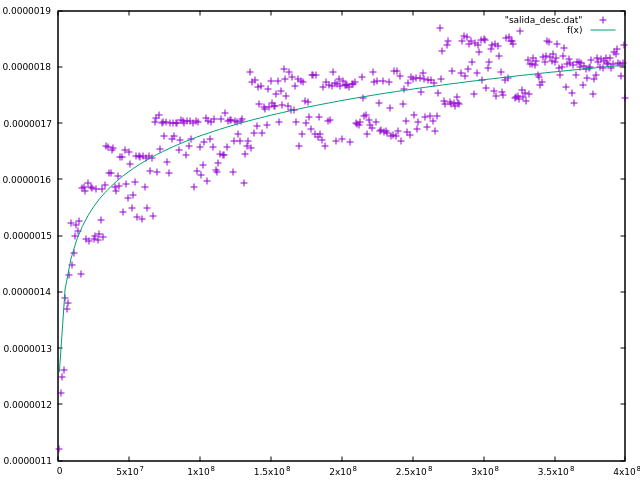
\includegraphics[width=0.5\textwidth]{./Imagenes/binaria_ajustada.png}
  \caption{Grafica de la salida de ejecuciones del algoritmo busqueda binaria}
\end{figure}

Si analizamos los siguientes datos se observa como al principio el tiempo de ejecucion crece mucho con cada incremento del tamaño de las entradas, pero luego apenas crece para aumentos de tamaño de 1000000 de datos, lo cual es un aumento considerable que no obstante apenas incrementa el tiempo de ejecución.

Además se ve como el tiempo de busqueda para un vector de tamaño 400000000 de datos es de menos de 0.0000019 segundos, lo cual denota que el algoritmo es muy rápido.

